\providecommand{\home}{../../..}
\documentclass[\home/main.tex]{subfiles}
\usetikzlibrary[arrows,snakes,backgrounds]
\usetikzlibrary{calc,positioning,fit}

\begin{document}

% \begin{sidewaysfigure}
\begin{tikzpicture}
    \def\picMinWidth{2.8cm}
    \def\picMinHeight{3.0cm}

    \tikzset{
        block/.append style={node distance=7.5mm,minimum width=3.5cm},
        subblock/.style={block, minimum width=1.5cm},
        picture/.style={block, node distance=6cm, fill=white, draw=white,minimum width=\picMinWidth, minimum height=\picMinHeight, text width=\picMinWidth,},
        preSpacedDash/.style={preSpaced, dashed,draw=black!50, thin},
        annot/.style={text width=4em, text centered},
    }

    \node[block] (env) {\includegraphics[width=\picMinWidth, height=\picMinHeight]{baxter_env_photo.JPG}};
    \node[below of=env, anchor=south, yshift=-1.25cm] (env_txt) {Image};

    \node[subblock, right= of env] (dnn) {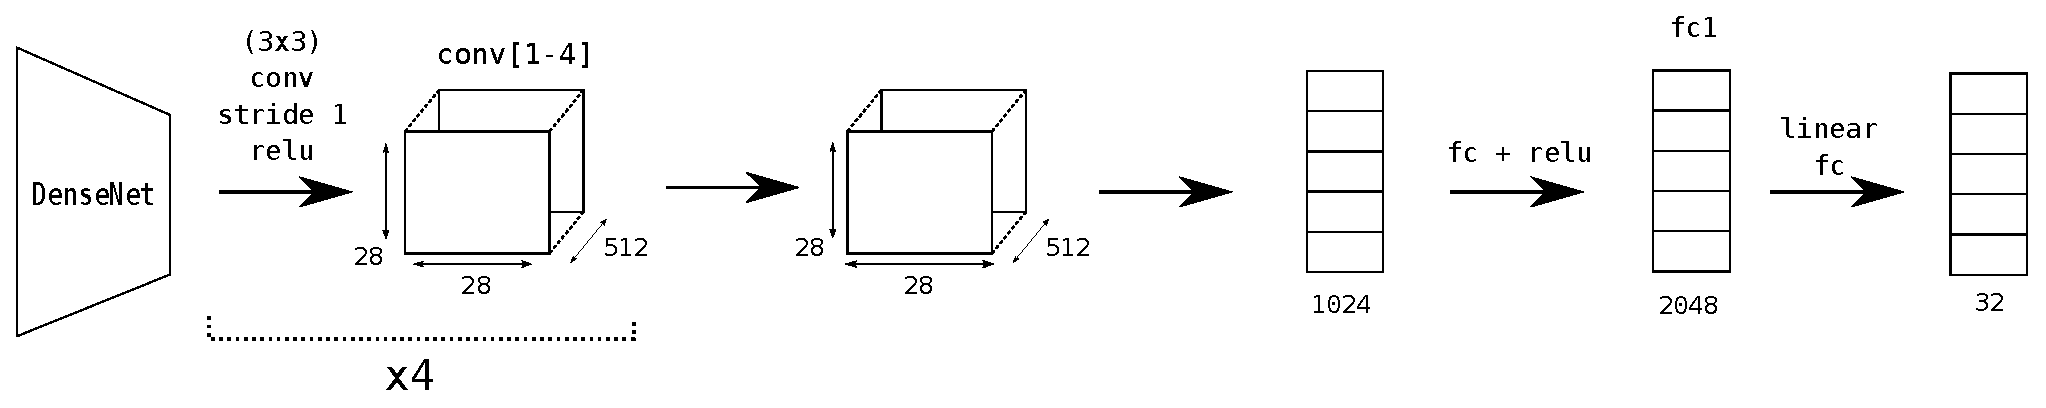
\includegraphics[width=11.5cm]{deep_nn_architecture.eps}};
    \node[below of=dnn, anchor=south, yshift=-1.0cm] (dnn_txt) {Deep neural network};
    \node[subblock,right=of dnn,align=center] (baxter) {Motor\\commands};

    \draw [postSpacedArrow] (env) to node [] {} (dnn);
    \draw [postSpacedArrow] (dnn) to node [] {} (baxter);

\end{tikzpicture}
% \end{sidewaysfigure}
\end{document}
